\documentclass[UTF8,fontset=none,aspectratio=169,10pt]{beamer}
\usepackage{ads-beamer-theme}

\title{高级分布式系统}
\subtitle{第五讲：术语、基本算法与分布式图算法}
\author{陈鹏飞\quad 计算机学院}
\institute{中山大学}
\date{2025--2026 学年}

\begin{document}

\begin{frame}[plain]
\begin{tikzpicture}[remember picture,overlay]
  \fill[ADSBlue] (current page.north west) rectangle ([xshift=2.4cm]current page.south west);
  \fill[ADSOrange] ([xshift=2.4cm]current page.north west) rectangle ([xshift=2.55cm]current page.south west);
  \node[anchor=west,align=left] at ([xshift=3.3cm,yshift=1.0cm]current page.west) {\fontsize{32}{38}\selectfont\color{ADSBlue}\bfseries 高级分布式系统};
  \node[anchor=west,align=left] at ([xshift=3.3cm,yshift=-0.4cm]current page.west) {\fontsize{21}{27}\selectfont\color{ADSDarkBlue}第五讲\quad 术语、基本算法与图算法};
  \node[anchor=west,align=left] at ([xshift=3.3cm,yshift=-2.2cm]current page.west) {\large\color{ADSGray}从拓扑抽象出发，构造生成树、最短路、MST、同步器与副本};
  \node[anchor=east] at ([xshift=-0.8cm,yshift=-3.2cm]current page.east) {\small\color{ADSGray}陈鹏飞\quad 中山大学\quad 2025--2026};
  \draw[ADSBlue,line width=0.8pt] ([xshift=3.3cm,yshift=-1.35cm]current page.west) -- ([xshift=12.6cm,yshift=-1.35cm]current page.west);
\end{tikzpicture}
\end{frame}

\long\def\latercontent{
\sectionframe{三、最短路与全源路径}{从局部邻居权重出发，反复应用三角不等式，把“我知道的路”变成全局最短路。}

\begin{frame}{同步单源最短路：Bellman--Ford}
\begin{itemize}
  \item 本例输入为无向加权图且不存在负权环；Bellman--Ford 本身也适用于有向图；
  \item 节点只知道 incident link 的权重，不知道全局图；
  \item 第 $k$ 轮结束时，节点得到至多经过 $k$ 条边的最短路径；
  \item 运行 $n-1$ 轮后稳定，假设节点知道 $n$ 才能按轮次终止；
  \item 每轮向所有邻居发送当前 distance，再按三角不等式更新。
\end{itemize}
\end{frame}

\begin{frame}{同步 Bellman--Ford：伪代码}
\scriptsize
\begin{block}{每个节点 $i$}
\begin{enumerate}
  \item $length\leftarrow\infty$；若 $i=i_0$，则 $length\leftarrow0$；
  \item 对 $round=1,\ldots,n-1$：向每个邻居发送 $UPDATE(i,length)$；
  \item 等待所有邻居的 UPDATE；
  \item 对每个邻居 $j$，若 $length>length_j+w_{j,i}$，则更新 $length\leftarrow length_j+w_{j,i}$，$parent\leftarrow j$。
\end{enumerate}
\end{block}
\normalsize
\vfill
\callout{消息}{每轮每条有向边一次 UPDATE，总计 $(n-1)|L|$ 量级。}
\end{frame}

\begin{frame}{Bellman--Ford 完整例子：距离如何逐轮传播}
\small
\begin{columns}[T,onlytextwidth]
\column{.37\textwidth}
\begin{block}{图与边权}
源点为 $s$：
\[
s\! -\! A:4,\quad s\! -\! B:1,\quad
B\! -\! A:2,
\]
\[
A\! -\! C:1,\quad B\! -\! C:5.
\]
每轮只使用上一轮邻居的距离：
\[
\begin{aligned}
d_v^{(r)}=\min\Bigl(&d_v^{(r-1)},\\[-1mm]
&\min_{u\in N(v)}\bigl[d_u^{(r-1)}+w(u,v)\bigr]\Bigr).
\end{aligned}
\]
\end{block}
\column{.59\textwidth}
\begin{center}
\begin{tabular}{c|cccc}
\toprule
轮次 & $d_s$ & $d_A$ & $d_B$ & $d_C$ \\
\midrule
0 & 0 & $\infty$ & $\infty$ & $\infty$ \\
1 & 0 & 4（经 $s$） & 1（经 $s$） & $\infty$ \\
2 & 0 & 3（经 $B$） & 1 & 5（经 $A$） \\
3 & 0 & 3 & 1 & 4（经 $A$） \\
\bottomrule
\end{tabular}
\end{center}
\begin{enumerate}
  \item 第 1 轮只发现一跳路径；
  \item 第 2 轮，$B$ 把更短的 $d_B=1$ 告诉 $A$；
  \item 第 3 轮，改进后的 $A$ 再把 $C$ 从 5 降到 4；
  \item 稳定后得到树边 $s\!\to B\!\to A\!\to C$。
\end{enumerate}
\end{columns}
\end{frame}

\begin{frame}{距离向量路由：Bellman--Ford 的持续版本}
\begin{itemize}
  \item 将标量 $length$ 替换为 $LENGTH[1..n]$，记录到每个目的地的最好估计；
  \item 将 $parent$ 替换为 $PARENT[1..n]$；
  \item 每次对每个目的地独立应用三角不等式；
  \item 链路权重可以是 RTT、排队延迟或负载，图会动态变化；
  \item 外层循环无限执行，直到路由稳定或发生下一次拓扑变化。
\end{itemize}
\vfill
\callout{风险}{异步更新可能产生 stale distance 和 count-to-infinity，必须配合 split horizon、序列号或毒性逆转。}
\end{frame}

\begin{frame}{异步单源最短路}
\begin{itemize}
  \item root 先广播 $UPDATE(i_0,0)$；
  \item 节点收到更短的估计才更新并向所有邻居继续传播；
  \item 无同步轮次，消息到达顺序决定中间状态；
  \item 一般最坏消息数和时间可能呈指数级；
  \item 若所有边权相等，算法退化为最少 hop 路由，计算所有目的地的 routing table 可用 $O(n^2|L|)$ 消息。
\end{itemize}
\end{frame}

\begin{frame}{Bellman--Ford 的不变量与课堂推演}
\begin{center}
\begin{tikzpicture}[node distance=8mm]
\nodebox{ADSBlue}{s}{源 $s$};
\nodebox[right=of s]{ADSOrange}{a}{局部估计 $d_a$};
\nodebox[right=of a]{ADSGreen}{b}{候选 $d_b+w_{ba}$};
\nodebox[right=of b]{ADSBlue}{new}{取较小值};
\draw[ADSBlue,\arrow] (s)--(a);
\draw[ADSOrange,\arrow] (a)--(b);
\draw[ADSGreen,\arrow] (b)--(new);
\end{tikzpicture}
\end{center}
\vfill
\begin{enumerate}
  \item 给一条含三条边的路径，逐轮写出 $length$；
  \item 将一个 UPDATE 延迟两个轮次，观察异步算法的中间估计；
  \item 讨论负权环为何破坏终止和稳定。
\end{enumerate}
\end{frame}

\begin{frame}{Floyd--Warshall：从单源到全源}
\begin{columns}[T,onlytextwidth]
\column{.48\textwidth}
\begin{itemize}
  \item 维护 $LENGTH[s,t]$ 和第一跳 $VIA[s,t]$；
  \item 外层 pivot 限制允许经过的中间节点集合；
  \item 若经 pivot 更短，则更新长度和第一跳。
\end{itemize}
\column{.47\textwidth}
\begin{block}{不变量}
经过 pivot 轮后，$LENGTH[s,t]$ 是只允许通过已处理 pivot 集合的最短路。
\end{block}
\begin{block}{集中式复杂度}
$O(n^3)$ 时间，矩阵空间 $O(n^2)$。
\end{block}
\end{columns}
\end{frame}

\begin{frame}{Floyd--Warshall 的三角不等式}
\begin{center}
\begin{tikzpicture}[node distance=9mm]
\nodebox{ADSBlue}{s2}{源 $s$};
\nodebox[above right=of s2]{ADSOrange}{piv}{pivot};
\nodebox[below right=of s2]{ADSOrange}{t2}{目的 $t$};
\draw[ADSBlue,\arrow] (s2)--(piv);
\draw[ADSBlue,\arrow] (piv)--(t2);
\draw[ADSGray,\arrow] (s2)--(t2);
\end{tikzpicture}
\end{center}
\vfill
\[
LENGTH[s,t]\leftarrow\min\{LENGTH[s,t],\;LENGTH[s,pivot]+LENGTH[pivot,t]\}.
\]
\vfill
\callout{VIA}{若更新发生，第一跳为 $VIA[s,pivot]$，而不是 pivot 本身。}
\end{frame}

\begin{frame}{分布式 Floyd--Warshall：行分片}
\begin{itemize}
  \item 节点 $i$ 存储矩阵的第 $i$ 行：$LEN[j]=LENGTH[i,j]$；
  \item $PARENT[j]$ 记录自己在以 $j$ 为 sink 的树上的 parent；
  \item 第 pivot 轮需要远程访问 $LENGTH[pivot,t]$，因此 pivot 行要沿 sink tree 分发；
  \item 所有节点必须在同一 pivot 上执行，否则不变量被破坏。
\end{itemize}
\vfill
\callout{关键}{分布式 Floyd--Warshall 本质上是“动态 sink tree + 每轮广播 + 局部三角不等式”。}
\end{frame}

\begin{frame}{动态 sink tree：父子发现}
\begin{center}
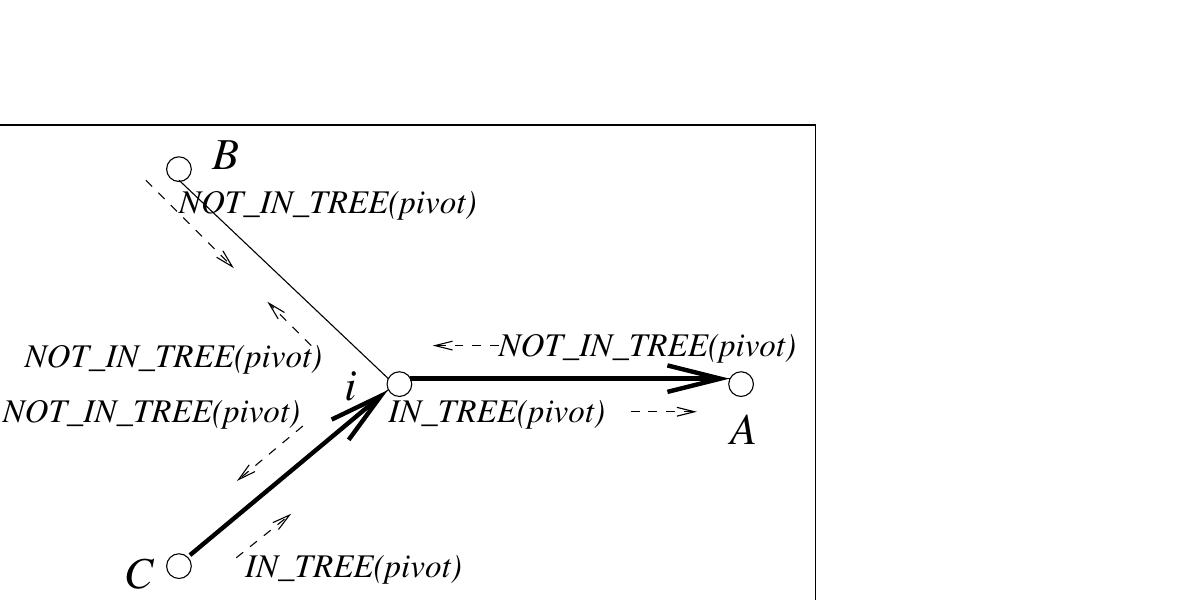
\includegraphics[width=.68\linewidth,height=.55\paperheight,keepaspectratio]{assets/week05-source-2025/sink-tree.png}
\end{center}
\smallnote{每轮 pivot，节点向 $PARENT[pivot]$ 发送 IN TREE，向其他邻居发送 NOT IN TREE；收到 IN TREE 的邻居就是当前 sink tree 的 child。}
\end{frame}

\begin{frame}{分布式 Floyd--Warshall：消息与同步}
\begin{itemize}
  \item 每轮先交换 IN TREE / NOT IN TREE，等待所有邻居回复；
  \item 若 $LEN[pivot]\neq\infty$，pivot 行沿 sink tree 向下广播；
  \item 收到整行后，每个节点执行局部三角不等式；
  \item 每轮的 send/receive 既标识树，也模拟 synchronizer 的安全点。
\end{itemize}
\vfill
\begin{tabularx}{\linewidth}{>{\bfseries}p{3.5cm}X}
\toprule
时间 & 每节点约 $O(n^2)$ 计算，加上 $n$ 次广播 \\
消息 & 总体 $O(n(|L|+n))$，PIV LEN 消息携带 $O(n)$ 数据 \\
\bottomrule
\end{tabularx}
\end{frame}

\begin{frame}{分布式 Floyd--Warshall：完整状态与消息}
\small
进程 $P_i$ 保存：
\begin{itemize}
  \item $LEN[1..n]$：$LEN[t]$ 是当前已知的 $i\rightarrow t$ 最短距离；初值为直连边权，$LEN[i]=0$，不可达为 $\infty$；
  \item $PARENT[1..n]$：$PARENT[t]$ 是 $P_i$ 在“以 $t$ 为 sink”的动态树上应把消息发给的下一跳；
  \item $Neighbours$、当前 $pivot$，以及收到的 \texttt{IN\_TREE}/\texttt{NOT\_IN\_TREE} 标记。
\end{itemize}
消息类型：
\begin{itemize}
  \item \texttt{IN\_TREE(pivot)}、\texttt{NOT\_IN\_TREE(pivot)}：发现当前 sink tree 的孩子；
  \item \texttt{PIV\_LEN(pivot,PIVOT\_ROW[1..n])}：携带 pivot 节点的整行距离。
\end{itemize}
\callout{读法}{$PARENT[pivot]$ 指向“怎样到达 pivot”；收到 \texttt{IN\_TREE} 的邻居则把本节点视为通往 pivot 的父节点。}
\end{frame}

\begin{frame}{分布式 Floyd--Warshall：完整中文伪代码}
\scriptsize
对 $pivot=1,\ldots,n$ 依次执行：
\begin{enumerate}
  \item 对每个邻居 $q$：若 $PARENT[pivot]=q$，发送 \texttt{IN\_TREE(pivot)}；否则发送 \texttt{NOT\_IN\_TREE(pivot)}。
  \item 等待每个邻居关于该 $pivot$ 的一条回复；收到 \texttt{IN\_TREE} 的邻居构成当前孩子集合。
  \item 若 $LEN[pivot]\neq\infty$：
    \begin{enumerate}
      \item 若 $pivot\neq i$，从 $PARENT[pivot]$ 接收 \texttt{PIV\_LEN}；若 $pivot=i$，令 $PIVOT\_ROW\leftarrow LEN$；
      \item 向每个孩子转发同一 $PIVOT\_ROW$；
      \item 对每个目的地 $t$，若
      \[
      LEN[pivot]+PIVOT\_ROW[t]<LEN[t],
      \]
      则令 $LEN[t]\leftarrow LEN[pivot]+PIVOT\_ROW[t]$，并令 $PARENT[t]\leftarrow PARENT[pivot]$。
    \end{enumerate}
\end{enumerate}
\smallnote{每轮必须等待树标记和 pivot 行到齐，才能进入下一 pivot；否则不同节点会混用不同阶段的数据，破坏 Floyd--Warshall 不变量。}
\end{frame}

\begin{frame}{约束泛洪：不建 spanning tree 也能传播}
\begin{itemize}
  \item FIFO 信道 + 序列号去重；
  \item 异步 flooding 常用于 IPv4 link-state routing；
  \item 一条源消息最坏约 $2|L|$ 条转发消息，时间约为 $d$ 个串行 hop；
  \item 同步版本可在 $d$ 轮后学习所有节点状态，但每条消息携带大小为 $n$ 的 STATEVEC；
  \item 代价是无需维护 ST，代价也转移到重复控制和大消息。
\end{itemize}
\end{frame}

\begin{frame}{异步 constrained flooding：序列号规则}
\scriptsize
\begin{block}{发送端}
root 每发送一条新消息 $M$，递增 $SEQNO[root]$，向所有邻居发送 $UPDATE(M,root,seq)$。
\end{block}
\begin{block}{接收端}
若收到的 $seq$ 大于本地记录：处理 $M$、更新序列号，并向除发送者外的邻居转发；否则丢弃重复消息。
\end{block}
\normalsize
\vfill
\callout{正确性}{同一个源的序列号在每个节点单调递增，保证重复包不会再次触发应用动作。}
\end{frame}

\begin{frame}{同步 constrained flooding：全局状态向量}
\begin{itemize}
  \item 每个节点把自己的局部值放入 $STATEVEC[i]$；
  \item 每轮向所有邻居发送整个向量；
  \item 收到邻居向量后做逐分量 max；
  \item $d$ 轮后每个节点都能学习全图的状态向量；
  \item 消息复杂度约为 $2|L|d$ 条、每条大小 $n$，时间复杂度 $d$ 轮。
\end{itemize}
\end{frame}

\sectionframe{四、GHS 最小生成树}{Kruskal 的“安全边”思想可以在没有全局排序的情况下，用 fragment 与 MWOE 并行实现。}

\begin{frame}{MST 基础：Kruskal 与 Prim}
\begin{columns}[T,onlytextwidth]
\column{.47\textwidth}
\blocktitle{Kruskal}
\begin{itemize}
  \item 维护森林；
  \item 每轮选连接两个不同分量的最小边；
  \item 集中式复杂度 $O(|L|\log |L|)$。
\end{itemize}
\column{.47\textwidth}
\blocktitle{Prim}
\begin{itemize}
  \item 从一个节点分量开始；
  \item 每轮选分量外接的最小边；
  \item 朴素 $O(n^2)$，堆优化可达 $O(n\log n)$。
\end{itemize}
\end{columns}
\vfill
\callout{分布式挑战}{每个节点只看到 incident edges，如何判断某条边连接的是同一分量？}
\end{frame}

\begin{frame}{GHS：fragment 与 MWOE（同步教学化版本）}
\begin{itemize}
  \item GHS 用 Kruskal 策略：初始每个节点是一个 fragment；
  \item MWOE（minimum weight outgoing edge）是从当前 fragment 指向其他 fragment 的最轻边；
  \item 把 fragment 的树与 MWOE 合并仍保持 spanning forest；
  \item 多个 fragment 可以并发选择 MWOE，每轮至少合并成对的 fragment；
  \item 在本页的同步 Borůvka 风格教学化轮次中，经过至多 $\lceil\log_2 n\rceil$ 轮得到一个 MST；标准 GHS 是带 level/phase 的异步协议，不能直接套用下面的轮次复杂度。
\end{itemize}
\end{frame}

\begin{frame}{MWOE：为什么安全}
\begin{center}
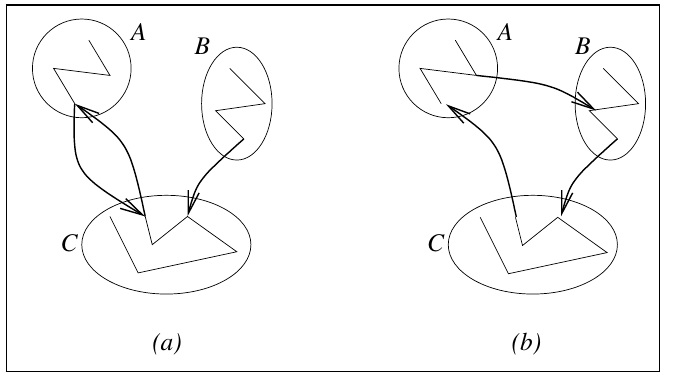
\includegraphics[width=.72\linewidth,height=.58\paperheight,keepaspectratio]{assets/week05-source-2025/mwoe-example-full.png}
\end{center}
\smallnote{对任一已有 spanning forest，某个 component 的最轻出边是安全边；若两端同时选择同一条边，合并不会产生环。}
\end{frame}

\begin{frame}{GHS 一轮的五个阶段}
\begin{enumerate}
  \item leader 在 fragment 树上 broadcast SEARCH MWOE；
  \item 每个节点沿非树边发送 EXAMINE，判断邻居是否属于其他 fragment；
  \item 节点把本地 MWOE convergecast 给 leader；
  \item leader 选全 fragment 的最小 MWOE，broadcast ADD MWOE；
  \item 两端都标记该边时，按端点 ID 选新 leader，并 broadcast NEW LEADER。
\end{enumerate}
\vfill
\callout{树角色}{marked edges 是 fragment 内的树边；unmarked edges 是待检查的 cross edges。}
\end{frame}

\begin{frame}{MST 例子：SEARCH、REPLY、ADD、NEW LEADER}
\begin{center}
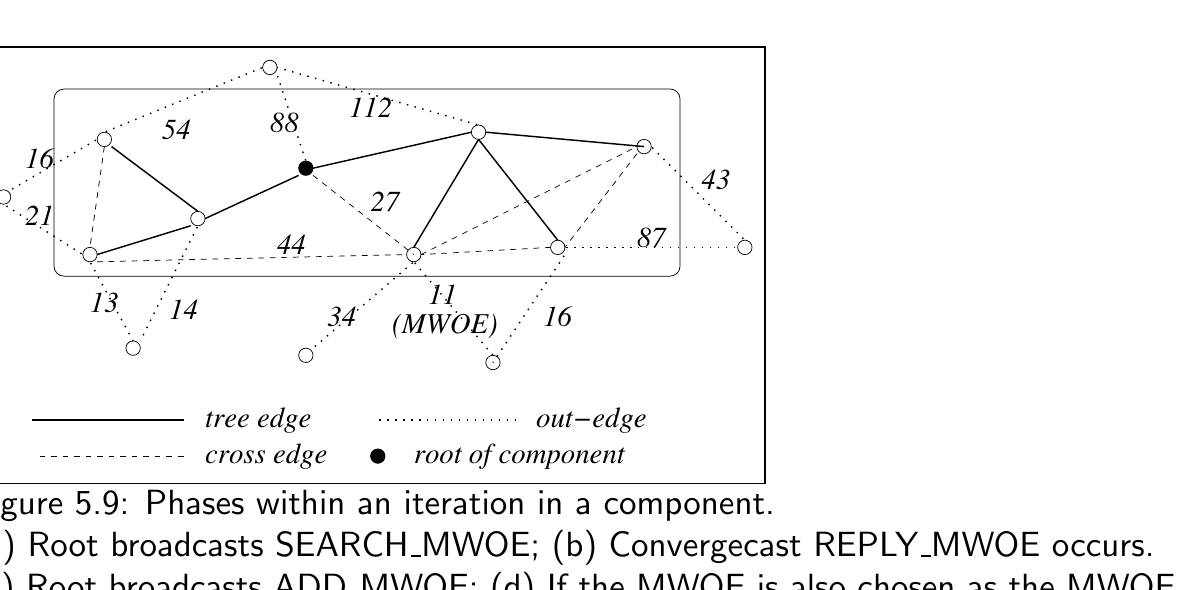
\includegraphics[trim=0 170 0 0,clip,width=.86\linewidth,height=.54\paperheight,keepaspectratio]{assets/week05-source-2025/mst-example.png}
\end{center}
\smallnote{实线为 fragment 内树边，虚线为 cross edge，点线为出边；黑点是当前 leader。图中最小权出边 $i_1$ 被汇总后选为 MWOE。}
\end{frame}

\begin{frame}{GHS 一轮完整例子：三个 fragment 如何合并}
\small
初始 fragment 为 $F_1=\{A,B\}$、$F_2=\{C,D\}$、$F_3=\{E,F\}$；
树边分别为 $AB(1),CD(2),EF(1)$，跨 fragment 边为
$BE(3),BC(4),DF(5),CE(6)$。
\begin{center}
\begin{tabularx}{.96\linewidth}{>{\bfseries}p{2.1cm}>{\raggedright\arraybackslash}X>{\raggedright\arraybackslash}X>{\raggedright\arraybackslash}X}
\toprule
阶段 & $F_1$ & $F_2$ & $F_3$ \\
\midrule
SEARCH/\newline EXAMINE & 比较 $BE(3),BC(4)$ & 比较 $BC(4),DF(5),CE(6)$ & 比较 $BE(3),DF(5),CE(6)$ \\
REPLY & MWOE=$BE(3)$ & MWOE=$BC(4)$ & MWOE=$BE(3)$ \\
ADD & 标记 $BE$ & 标记 $BC$ & 标记 $BE$ \\
\bottomrule
\end{tabularx}
\end{center}
\begin{enumerate}
  \item $F_1$ 与 $F_3$ 双方都选择 $BE(3)$，先合成 $F_{13}$；
  \item $F_2$ 通过安全边 $BC(4)$ 接入 $F_{13}$；
  \item 新 fragment 用端点 ID 规则选 leader，并广播 NEW LEADER；
  \item 加入的两条边连接不同 fragment，不会产生环。
\end{enumerate}
\end{frame}

\begin{frame}{Sync GHS：消息类型}
\scriptsize
\begin{tabularx}{\linewidth}{>{\ttfamily\bfseries}p{3.9cm}X}
\toprule
SEARCH MWOE(leader) & 沿 marked tree broadcast，开启本轮搜索 \\
EXAMINE(leader) & 沿 unmarked edge 判断另一端 fragment \\
REPLY MWOES(local,remote) & 节点向 leader 汇报本地最轻出边 \\
ADD MWOE(local,remote) & leader 选择并标记要加入 MST 的边 \\
NEW LEADER(leader) & 合并后向新 fragment 广播 leader \\
\bottomrule
\end{tabularx}
\normalsize
\end{frame}

\begin{frame}{Sync GHS：完整中文伪代码（搜索与汇聚）}
\scriptsize
初始化：每个节点令 $leader\leftarrow i$；执行至多 $\lceil\log_2 n\rceil$ 轮。
\begin{enumerate}
  \item 若本节点是 leader，沿 fragment 的 marked tree edges 广播 \texttt{SEARCH MWOE(leader)}。
  \item 节点收到 SEARCH 后，沿每条 unmarked edge 发送 \texttt{EXAMINE(leader)}，比较对端 leader：
  \begin{itemize}\scriptsize
    \item 对端 leader 相同：该边是 fragment 内部边，不参加本轮候选；
    \item 对端 leader 不同：该边是 outgoing edge，参与本地最小值比较。
  \end{itemize}
  \item 每个节点选出本地最轻 outgoing edge，记为 $MWOE_i=(localID,remoteID,weight)$。
  \item fragment 树的叶节点先发送 \texttt{REPLY MWOES}；内部节点等待所有孩子回复，将孩子候选与 $MWOE_i$ 取最小后继续 convergecast。
\end{enumerate}
\normalsize
\vfill
\callout{为什么要汇聚}{leader 必须比较整个 fragment 的所有边界候选，局部最轻边不一定是 fragment 的全局 MWOE。}
\end{frame}

\begin{frame}{Sync GHS：完整中文伪代码（合并与新 leader）}
\scriptsize
\begin{enumerate}
  \item leader 收齐 convergecast 后，选择全 fragment 的最小 $MWOE=(u,v,w)$。
  \item leader 沿 marked tree 广播 \texttt{ADD MWOE(u,v)}，直到端点 $u$；$u$ 请求把边 $(u,v)$ 标为树边。
  \item 若 $(u,v)$ 两端所属 fragment 都选择了该边，则两边同时标记并完成合并；若只有一侧选择，则等待另一 fragment 的兼容合并动作。
  \item 合并后，以端点 ID 的确定性规则选择新 leader，例如 $\max(u,v)$。
  \item 新 leader 沿新 fragment 的全部 marked edges 广播 \texttt{NEW LEADER(newLeader)}；所有节点更新 leader，进入下一轮。
\end{enumerate}
\normalsize
\vfill
\callout{正确性直觉}{MWOE 是跨越当前 cut 的安全边；确定性 leader 规则只负责统一控制者，不改变安全边性质。}
\end{frame}

\begin{frame}{Sync GHS：复杂度与同步必要性（仅适用于本页简化模型）}
\begin{tabularx}{\linewidth}{>{\bfseries}p{3.3cm}X}
\toprule
轮数 & $O(\log n)$ \\
时间 & $O(n\log n)$（按 fragment 树高上界） \\
消息 & 每轮树边 $O(n)$，EXAMINE 为 $|L|$，总计 $O((n+|L|)\log n)$ \\
\bottomrule
\end{tabularx}
\vfill
\begin{itemize}
  \item EXAMINE 要比较两端 fragment level/leader；
  \item 若两端处于不同轮次，旧 leader 可能误答“同 fragment”；
  \item 可能把 cross edge 当作树边，进而产生环。
\end{itemize}
\end{frame}

\begin{frame}{异步 GHS：用同步器模拟，还是重新设计？}
\begin{itemize}
  \item 直接在同步 GHS 外包 synchronizer，需要额外 ACK、round 和 level 消息；
  \item 新 leader 需在 marked edges 上做 BC/CC，确保邻居知道新轮次；
  \item 额外开销约为 $n\log n$ 条级别的控制消息，非树边还需 $|L|\log n$ 级别的通知；
  \item 工程化异步 GHS 的目标可以是消息 $O(n\log n+|L|)$、时间 $O(n\log n(|L|+d))$；
  \item 难点：不同 level 的 fragment 如何协调 MWOE 搜索与合并？
\end{itemize}
\end{frame}

\sectionframe{五、Synchronizer：在异步系统中模拟轮次}{用安全条件把“下一轮”变成可验证事件，为已有同步算法提供异步运行时。}

\begin{frame}{Synchronizer 的定义}
\begin{itemize}
  \item synchronizer 是一种变换算法，让为同步系统设计的程序在异步系统上运行；
  \item 假设系统无故障；有时从头写异步算法更高效；
  \item process $i$ 在 round $r$ 安全，当它发出的该轮消息都已被接收；
  \item 核心：通知节点何时所有应接收的消息已到达，可以进入下一轮。
\end{itemize}
\end{frame}

\begin{frame}{Synchronizer 的统一成本公式}
\[
M_a=M_s+(M_{init}+rounds\cdot M_{round}),
\qquad
T_a=T_s+T_{init}+rounds\cdot T_{round}.
\]
\begin{tabularx}{\linewidth}{>{\bfseries}p{3cm}X}
\toprule
$M_s,T_s$ & 原同步算法的消息数和时间 \\
$M_{init},T_{init}$ & 初始化异步系统的消息/串行 hop \\
$M_{round},T_{round}$ & 模拟一个同步轮次的额外成本 \\
\bottomrule
\end{tabularx}
\end{frame}

\begin{frame}{三类 synchronizer 的比较}
\begin{tabularx}{\linewidth}{>{\bfseries}p{2.7cm}XXXX}
\toprule
 & Simple & $\alpha$ & $\beta$ / cluster \\
\midrule
$M_{init}$ & 0 & 0 & $O(n\log n+|L|)$ \\
$T_{init}$ & $d$ & 0 & $O(n)$ \\
$M_{round}$ & $2|L|$ & $O(|L|)$ & $O(n)$ 或 $O(L_c)$ \\
$T_{round}$ & 1 & $O(1)$ & $O(n)$ 或 $O(h_c)$ \\
\bottomrule
\end{tabularx}
\vfill
\smallnote{$h_c$ 为 cluster tree 最大高度，$L_c$ 为 cluster 内树边与 designated inter-cluster 边总数。}
\end{frame}

\begin{frame}{Simple synchronizer}
\begin{center}
\begin{tikzpicture}[node distance=9mm and 16mm,>=Latex]
  \nodebox{ADSBlue}{pi}{$P_i$\\第 $r$ 轮};
  \nodebox[right=of pi]{ADSOrange}{pj}{$P_j$\\第 $r$ 轮};
  \draw[\arrow,ADSBlue] (pi.north east) to[bend left=18] node[above]{本轮消息或 dummy}(pj.north west);
  \draw[\arrow,ADSOrange] (pj.south west) to[bend left=18] node[below]{本轮消息或 dummy}(pi.south east);
  \nodebox[below=18mm of pi]{ADSGreen}{pin}{$P_i$\\进入第 $r+1$ 轮};
  \nodebox[below=18mm of pj]{ADSGreen}{pjn}{$P_j$\\进入第 $r+1$ 轮};
  \draw[\arrow,ADSGreen] (pi)--node[left]{收齐邻居}(pin);
  \draw[\arrow,ADSGreen] (pj)--node[right]{收齐邻居}(pjn);
\end{tikzpicture}
\end{center}
\smallnote{即使本轮没有真实数据，也要发送 dummy，证明“我在本轮不会再发消息”。相邻节点的轮次最多相差 1。}
\end{frame}

\begin{frame}{Simple synchronizer：安全性与初始化}
\begin{itemize}
  \item 相邻节点的轮次最多相差 1；处于 round $r$ 的节点只会收到邻居 round $r$ 或 $r+1$ 的消息；
  \item 任意节点可从 round $x$ 开始；经过 $d$ 个消息 hop，所有节点都达到 round $x$；
  \item $M_{init}=0$，$T_{init}=d$；
  \item 每轮 $M_{round}=2|L|$，$T_{round}=1$。
\end{itemize}
\end{frame}

\begin{frame}{$\alpha$ synchronizer：ACK 与 safe}
\begin{columns}[T,onlytextwidth]
\column{.50\textwidth}
\begin{center}
\begin{tikzpicture}[node distance=13mm,>=Latex]
  \nodebox{ADSBlue}{pa}{$P_i$};
  \nodebox[right=of pa]{ADSOrange}{pb}{$P_j$};
  \draw[\arrow,ADSBlue] (pa.north east) to[bend left=18] node[above]{第 $r$ 轮消息}(pb.north west);
  \draw[\arrow,ADSGreen] (pb.south west) to[bend left=18] node[below]{ACK}(pa.south east);
  \nodebox[below=16mm of pa,minimum width=4.4cm]{ADSGreen}{safe}{本地消息均获 ACK\\宣布本轮 safe};
  \draw[\arrow,ADSGreen] (pa)--(safe);
\end{tikzpicture}
\end{center}
\column{.45\textwidth}
\begin{itemize}
  \item 节点收到邻居对本轮每条消息的 ACK 后，宣布自己 safe；
  \item 当邻居都 safe，节点才进入下一轮；
  \item transport layer ACK 可视为“免费”，但 safe 通知仍需传播；
  \item 每轮约 $2|L|$ 条 safe 消息，$O(1)$ 个串行 hop。
\end{itemize}
\end{columns}
\end{frame}

\begin{frame}{$\beta$ synchronizer：根树上的 CvgC/BC}
\begin{itemize}
  \item 预先建立 rooted spanning tree；初始化约 $O(n\log n+|L|)$ 消息、$O(n)$ 时间；
  \item 安全节点发起 convergecast，子树全部安全后向上转发；
  \item root 收到所有 child 的 CvgC 后，在树上 broadcast，通知所有节点进入下一轮；
  \item 每轮 $2(n-1)$ 条树消息，平均 $2\log n$ hop，最坏 $2n$ hop。
\end{itemize}
\end{frame}

\begin{frame}{Cluster synchronizer：局部快、全局稳}
\begin{center}
\begin{tikzpicture}[node distance=8mm and 16mm,>=Latex]
  \node[draw=ADSBlue,rounded corners,minimum width=4cm,minimum height=2.2cm,label=above:{Cluster A：内部 $\beta$ 同步}] (ca) {};
  \node[draw=ADSOrange,rounded corners,right=of ca,minimum width=4cm,minimum height=2.2cm,label=above:{Cluster B：内部 $\beta$ 同步}] (cb) {};
  \foreach \x/\y in {-.9/.35,0/.7,.9/.35,-.45/-.55,.45/-.55}{\fill[ADSBlue] ($(ca.center)+(\x,\y)$) circle (2.2pt);}
  \foreach \x/\y in {-.9/.35,0/.7,.9/.35,-.45/-.55,.45/-.55}{\fill[ADSOrange] ($(cb.center)+(\x,\y)$) circle (2.2pt);}
  \draw[ADSBlue] ($(ca.center)+(0,.7)$)--($(ca.center)+(-.9,.35)$)--($(ca.center)+(-.45,-.55)$);
  \draw[ADSBlue] ($(ca.center)+(0,.7)$)--($(ca.center)+(.9,.35)$)--($(ca.center)+(.45,-.55)$);
  \draw[ADSOrange] ($(cb.center)+(0,.7)$)--($(cb.center)+(-.9,.35)$)--($(cb.center)+(-.45,-.55)$);
  \draw[ADSOrange] ($(cb.center)+(0,.7)$)--($(cb.center)+(.9,.35)$)--($(cb.center)+(.45,-.55)$);
  \draw[very thick,ADSGreen,dashed,\arrow] ($(ca.center)+(.9,.35)$)--node[above]{指定的跨 cluster 边：$\alpha$ 同步}($(cb.center)+(-.9,.35)$);
\end{tikzpicture}
\end{center}
\smallnote{cluster 内沿树做 CvgC/BC；相邻 cluster 之间只选择一条代表边交换 safe 状态，避免所有跨域链路都参与。}
\end{frame}

\begin{frame}{Cluster synchronizer：运行与复杂度}
\begin{itemize}
  \item cluster 内先用树同步器推进；
  \item cluster 稳定后，在 designated edge 上运行 $\alpha$ synchronizer；
  \item inter-cluster 稳定后，再由 cluster 内 CvgC/BC 传播稳定信号；
  \item 每轮消息 $M_{round}=O(L_c)$，时间 $T_{round}=O(h_c)$；
  \item 适合数据中心中“机架内高速、机架间慢”的分层网络。
\end{itemize}
\end{frame}

\sectionframe{六、MIS、CDS 与压缩路由}{从局部随机优先级中选出互不相邻节点，再把它们连接成广播骨干或压缩转发表。}

\begin{frame}{Maximal Independent Set（MIS）}
\begin{itemize}
  \item 独立集 $N'\subseteq N$：任意 $i,j\in N'$ 之间没有边；
  \item maximal：不能再加入任何节点；
  \item maximum：大小最大的 independent set，通常是 NP-complete；
  \item 应用：无线广播、频段分配和局部互斥。
\end{itemize}
\vfill
\callout{区分}{maximal 只要求“不能扩展”，不要求“规模最大”。}
\end{frame}

\begin{frame}{Luby 随机 MIS：每轮逻辑}
\begin{enumerate}
  \item 每个候选节点随机选一个足够大的数并发送给邻居；
  \item 若自己的数在邻域中最低，则加入 MIS；
  \item MIS 节点通知邻居，邻居退出候选集；
  \item 未被选中的节点继续下一轮；
  \item 期望每轮至少消除常数比例节点，期望轮数 $O(\log n)$。
\end{enumerate}
\vfill
\callout{正确性}{选中节点之间不相邻；任何未选节点最终都邻接一个已选节点，因此集合 maximal。}
\end{frame}

\begin{frame}{Luby MIS：完整中文伪代码（随机竞争）}
\scriptsize
状态：候选邻居集合 $Neighbours$，随机数 $random_i$，布尔量 $selected_i,eliminated_i$。
\begin{enumerate}
  \item 重复执行；若 $Neighbours=\varnothing$，令 $selected_i\leftarrow true$ 并结束。
  \item 生成随机数 $random_i$，向所有候选邻居发送 \texttt{RANDOM(random$_i$)}。
  \item 等待每个 $j\in Neighbours$ 的随机数；若 $(random_i,i)$ 按字典序小于所有 $(random_j,j)$：
  \begin{itemize}\scriptsize
    \item 向所有邻居发送 \texttt{SELECTED(i,true)}；
    \item 令 $selected_i\leftarrow true$，作为 MIS 成员结束。
  \end{itemize}
  \item 否则向所有邻居发送 \texttt{SELECTED(i,false)}，等待本轮所有 SELECTED 消息。
\end{enumerate}
\normalsize
\smallnote{字典序 tie-break 补足原算法中“随机数范围足够大”的工程假设，避免平局造成相邻节点同时入选。}
\end{frame}

\begin{frame}{Luby MIS：完整中文伪代码（淘汰与进入下一轮）}
\scriptsize
\begin{enumerate}
  \item 若从某个邻居收到 \texttt{SELECTED(j,true)}：
  \begin{itemize}\scriptsize
    \item 自己不能进入 MIS，令 $eliminated_i\leftarrow true$；
    \item 通知仍是候选的邻居自己已被淘汰，然后结束。
  \end{itemize}
  \item 若本轮没有任何邻居被选中：
  \begin{itemize}\scriptsize
    \item 向所有候选邻居发送 \texttt{ELIMINATED(i,false)}；
    \item 等待邻居的 ELIMINATED 状态；
    \item 对每个返回 \texttt{ELIMINATED(j,true)} 的邻居，从 $Neighbours$ 中删除 $j$。
  \end{itemize}
  \item 使用缩小后的候选邻居集合进入下一轮。
\end{enumerate}
\normalsize
\vfill
\callout{两条性质}{相邻节点不会同时 selected，保证 independent；退出的节点必邻接某个 selected 节点，最终保证 maximal。}
\end{frame}

\begin{frame}{Luby MIS：图例}
\begin{center}
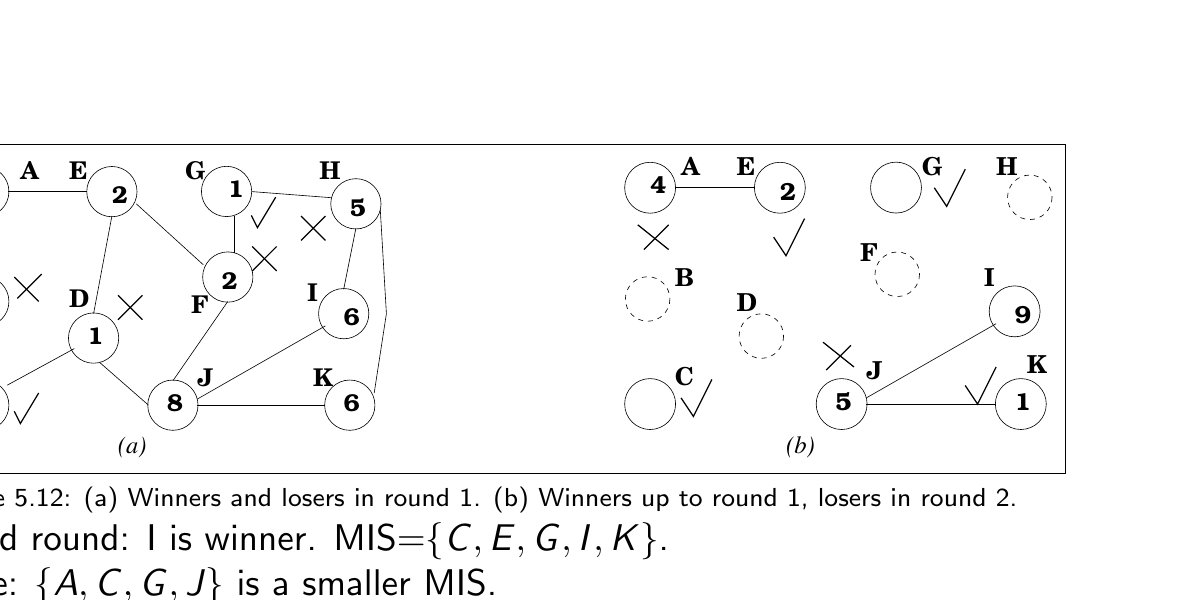
\includegraphics[trim=0 82 0 0,clip,width=.74\linewidth,height=.56\paperheight,keepaspectratio]{assets/week05-source-2025/mis-example.png}
\end{center}
\smallnote{示例的最终 MIS 为 $\{C,E,G,I,K\}$；$\{A,C,G,J\}$ 也可能是较小的 maximal independent set。}
\end{frame}

\begin{frame}{Connected Dominating Set（CDS）}
\begin{itemize}
  \item dominating set：每个不在集合中的节点至少有一个邻居在集合中；
  \item CDS：诱导子图还必须连通；
  \item minimum CDS 是 NP-complete，工程上使用近似和启发式；
  \item 常见构造：先建 spanning tree 再删叶子，或先建 MIS 再加边连接 MIS 节点；
  \item 应用：无线/数据中心广播骨干、故障域覆盖和控制平面中继。
\end{itemize}
\end{frame}

\begin{frame}{Compact routing：为什么压缩转发表}
\begin{center}
\begin{tikzpicture}[x=1.25cm,y=1.1cm,>=Latex]
  \node[circle,draw=ADSBlue] (n4) at (3,2.4) {4};
  \node[circle,draw=ADSBlue] (n2) at (1.5,1.2) {2};
  \node[circle,draw=ADSBlue] (n6) at (4.5,1.2) {6};
  \node[circle,draw=ADSGray] (n1) at (.5,0) {1};
  \node[circle,draw=ADSGray] (n3) at (2.2,0) {3};
  \node[circle,draw=ADSGray] (n5) at (3.8,0) {5};
  \node[circle,draw=ADSGray] (n7) at (5.5,0) {7};
  \draw[ADSBlue] (n4)--node[above left]{目的区间 $[1,3]$}(n2);
  \draw[ADSBlue] (n4)--node[above right]{目的区间 $[5,7]$}(n6);
  \draw[ADSGray] (n2)--node[left]{$[1,1]$}(n1);
  \draw[ADSGray] (n2)--node[right]{$[3,3]$}(n3);
  \draw[ADSGray] (n6)--node[left]{$[5,5]$}(n5);
  \draw[ADSGray] (n6)--node[right]{$[7,7]$}(n7);
  \node[anchor=west,align=left] at (6.3,1.7){完整转发表：每个目的地一项\\区间路由：连续目的地共享一项\\代价：路径可能拉长或流量失衡};
\end{tikzpicture}
\end{center}
\smallnote{完整表大小为 $n$ 会增加内存和查表时间；树标签和区间标签用地址区间压缩目的地集合，但可能造成流量不均衡。}
\end{frame}

\begin{frame}{Interval routing 与 prefix routing}
\begin{itemize}
  \item 节点标签 $B$ 是 $N$ 的一一映射；
  \item 每条出边标注若干目的地标签，覆盖所有目的地且互不重复；
  \item 对任意 $s,t$，沿路径逐跳选择包含 $B(t)$ 的边标签；
  \item interval labeling 对任意图都可构造，但不保证路径长度，也不适应频繁拓扑变化；
  \item prefix routing 把节点/信道标签视为字符串，选择与目的地址最长匹配的出边。
\end{itemize}
\end{frame}

\begin{frame}{Stretch factor：压缩的代价}
\[
stretch(r)=\max_{i,j\in N}\frac{distance_r(i,j)}{distance_{opt}(i,j)}.
\]
\begin{itemize}
  \item 分子是路由方案的路径长度，分母是最优路径长度；
  \item stretch 越小，路由越接近最短路；
  \item grid、ring、tree 等特殊拓扑有更容易证明的 compact routing 结果；
  \item AI 集群中可将 stretch 与 GPU 间带宽、拥塞和尾延迟联合优化。
\end{itemize}
\end{frame}

\sectionframe{七、选主与自适应复制}{最后把“全局一致的一个节点”与“随访问热度移动的多个副本”放在同一条控制平面上。}

\begin{frame}{Leader election：问题定义}
\begin{itemize}
  \item 所有进程最终同意一个 distinguished process；
  \item 分布式算法通常需要 initiator 和 finisher，即使它们运行同样代码；
  \item 无 ID 的匿名环上不存在确定性选主；
  \item 本讲先看异步单向环上的 LCR，再看 Hirschberg--Sinclair 的加速。
\end{itemize}
\end{frame}

\begin{frame}{LCR：最高 ID 在环上胜出}
\begin{itemize}
  \item 每个节点把自己的 ID 作为 PROBE 沿右邻居发送；
  \item 收到比自己大的 ID 就转发，比自己小的就丢弃；
  \item 自己的 ID 绕环一周回来，说明它是最高 ID；
  \item 发送 SELECTED(ID) 一周，所有节点记录 leader；
  \item 在可靠单向环、每跳有界且每个节点同时发起一次的模型下，消息复杂度最坏 $n(n-1)/2$，时间复杂度按环跳数为 $O(n)$。
\end{itemize}
\end{frame}

\begin{frame}{LCR：完整中文伪代码}
\scriptsize
状态：$participate=false$；消息类型为 \texttt{PROBE(id)} 与 \texttt{SELECTED(id)}。
\begin{enumerate}
  \item 唤醒：发送 PROBE(i)，$participate\leftarrow true$；
  \item 收到 PROBE(k)：若 $i>k$ 丢弃；若 $i<k$ 转发；若 $i=k$ 宣布 leader 并发 SELECTED(i)；
  \item 收到 SELECTED(x)：若 $x\neq i$，记录并转发；若 $x=i$，停止转发；
  \item 节点可延迟参与，收到 probe 后先执行唤醒动作。
\end{enumerate}
\normalsize
\end{frame}

\begin{frame}{LCR 完整例子：ID 9 如何绕环胜出}
\small
单向环为 $P_7\rightarrow P_2\rightarrow P_9\rightarrow P_4\rightarrow P_7$。
\begin{center}
\begin{tabularx}{.96\linewidth}{>{\bfseries}p{1.6cm}X}
\toprule
步骤 & 消息变化 \\
\midrule
初始化 & 每个节点发送自己的 PROBE：$7,2,9,4$。 \\
第 1 跳 & $P_2$ 转发 7；$P_9$ 丢弃 2；$P_4$ 转发 9；$P_7$ 丢弃 4。 \\
第 2 跳 & $P_9$ 丢弃 7；$P_7$ 看到 $9>7$，继续转发 9。 \\
第 3 跳 & $P_2$ 继续转发 9。 \\
第 4 跳 & $P_9$ 收到自己的 9，确认环中不存在更大 ID。 \\
宣布 & $P_9$ 发送 SELECTED(9) 一周，所有节点记录 leader=9。 \\
\bottomrule
\end{tabularx}
\end{center}
\callout{为什么正确}{较小 ID 的 probe 遇到较大 ID 就被吸收；只有全局最大 ID 能完整绕环返回发送者。}
\end{frame}

\begin{frame}{Hirschberg--Sinclair：指数半径淘汰}
\begin{itemize}
  \item 第 $k$ 轮，活跃节点向两个方向探测半径 $2^k$；
  \item 若自己是半径内最高 ID，才进入下一轮；
  \item 每轮候选者间距至少 $2^k$，候选数按对数下降；
  \item $O(\log n)$ 轮，每轮最多 $O(n)$ 消息，总消息 $O(n\log n)$；
  \item 时间仍为 $O(n)$，但消息量相对 LCR 大幅降低。
\end{itemize}
\end{frame}

\begin{frame}{对象复制：从最优放置到自适应}
\begin{itemize}
  \item 图 $G=(N,L)$ 上有用户节点集合 $N_k$ 和副本节点集合 $N_r$；
  \item 只读访问时，目标是最小化用户到最近副本的距离总和；
  \item 若读频率不同，距离项要乘用户权重；
  \item 更新操作需要同步所有副本，写多时副本越多越贵；
  \item 任意图上的最优复制是 NP-complete，因此转向 tree overlay 上的自适应近似。
\end{itemize}
\end{frame}

\begin{frame}{Adaptive Data Replication：目标函数}
设 $r_i,w_i$ 为节点 $i$ 的读/写速率，$c_r(i),c_w(i)$ 为相应成本，复制方案为 $R$：
\[
\min_{R\in\mathcal R}\left[\sum_{i\in V}r_i c_r(i)+\sum_{i\in V}w_i c_w(i)\right].
\]
\begin{itemize}
  \item 使用 ROWA（Read-One-Write-All）保证 one-copy serializability；
  \item 读从最近副本获得，写先到最近副本，再在 $R$ 内传播；
  \item 读热点使 $R$ 扩张，写热点使 $R$ 收缩。
\end{itemize}
\end{frame}

\begin{frame}{树 overlay 上的“变形虫”副本集合}
\begin{center}
\begin{tikzpicture}[scale=.80,transform shape,node distance=7mm and 12mm,>=Latex]
  \nodebox{ADSGray}{a}{A};
  \nodebox[right=of a]{ADSGreen}{b}{B：副本};
  \nodebox[right=of b]{ADSGreen}{c}{C：副本};
  \nodebox[above right=of c]{ADSGreen}{d}{D：副本};
  \nodebox[below right=of c]{ADSGray}{e}{E};
  \nodebox[right=of d]{ADSGray}{f}{F};
  \draw[ADSGray] (a)--(b);
  \draw[very thick,ADSGreen] (b)--(c)--(d);
  \draw[ADSGray] (c)--(e);
  \draw[ADSGray] (d)--(f);
  \node[draw=ADSGreen,dashed,rounded corners,fit=(b)(c)(d),inner sep=5mm,label=above:{$R$：连通副本子图}] {};
\end{tikzpicture}
\end{center}
\smallnote{$R$ 是树上的连通子图，随读写活动中心移动；通信只沿树边和 $R$ 的邻居关系发生。}
\end{frame}

\begin{frame}{R-neighbour 与 R-fringe}
\begin{columns}[T,onlytextwidth]
\column{.46\textwidth}
\begin{itemize}
  \item R-neighbour：$i\in R$ 且至少有一个邻居不在 $R$；
  \item R-fringe：$i\in R$ 且只有一个邻居在 $R$，即 $R$ 子图中的叶子；
  \item singleton：$|R|=1$。
\end{itemize}
\column{.50\textwidth}
\begin{tikzpicture}[scale=.70,transform shape,node distance=5mm and 7mm,>=Latex]
  \nodebox{ADSGreen}{x}{内部副本};
  \nodebox[right=of x]{ADSOrange}{y}{边界副本};
  \nodebox[right=of y]{ADSGray}{z}{非副本邻居};
  \nodebox[below=of y]{ADSBlue}{p}{唯一内部邻居};
  \draw[very thick,ADSGreen] (x)--(y);
  \draw[ADSGray] (y)--(z);
  \draw[very thick,ADSGreen] (y)--(p);
  \node[below=10mm of z,align=center]{边界副本有外部邻居：\\R-neighbour};
  \node[below=10mm of x,align=center]{在 $R$ 中只有一个邻居：\\R-fringe};
\end{tikzpicture}
\end{columns}
\end{frame}

\begin{frame}{三个 epoch 测试}
\begin{tabularx}{\linewidth}{>{\bfseries}p{2.6cm}X}
\toprule
Expansion & R-neighbour 节点把邻居 $j$ 加入 $R$，若从 $j$ 方向收到的读多于本地和其他方向的写。 \\
Contraction & R-fringe 节点退出 $R$，若唯一内部邻居方向的写多于本地和其他方向的读；退出前需获许可，避免 $R=\emptyset$。 \\
Switch & singleton 将副本转移给更热的邻居，比较各方向的读写总和。 \\
\bottomrule
\end{tabularx}
\vfill
\callout{顺序}{R-neighbour 可能同时是 fringe；先做 expansion，失败后再做 contraction 或 switch。}
\end{frame}

\begin{frame}{Adaptive replication：扩张与收缩图示}
\begin{center}
\begin{tikzpicture}[node distance=8mm and 15mm,>=Latex]
  \nodebox{ADSGreen}{r1}{副本 $i$};
  \nodebox[right=of r1]{ADSGray}{n1}{读热点 $j$};
  \draw[very thick,ADSOrange,\arrow] (n1)--node[above]{读量高}(r1);
  \node[below=8mm of $(r1)!0.5!(n1)$]{Expansion：把 $j$ 加入 $R$};
  \nodebox[below=22mm of r1]{ADSGreen}{r2}{边缘副本 $i$};
  \nodebox[right=of r2]{ADSGreen}{in2}{内部副本 $j$};
  \draw[very thick,ADSBlue,\arrow] (in2)--node[above]{写量高}(r2);
  \node[below=8mm of $(r2)!0.5!(in2)$]{Contraction：$i$ 获许可后退出 $R$};
\end{tikzpicture}
\end{center}
\smallnote{热点方向会吸引副本，写热点会把副本边界推回；稳定访问模式下，$d+1$ 个 epoch 内可收敛到平衡状态。}
\end{frame}

\begin{frame}{Adaptive replication：完整中文伪代码（测试调度）}
\small
每个 epoch 结束时，$P_i$ 根据自己在 $R$ 中的位置选择测试：
\begin{enumerate}
  \item 若同时是 R-neighbour 与 R-fringe：先做 expansion；若没有扩张，再做 contraction；
  \item 若 $|R|=1$（singleton）：先尝试向热点邻居 expansion；失败后再做 switch；
  \item 若是 R-neighbour，但既非 fringe 也非 singleton：只做 expansion；
  \item 若是 R-fringe 但没有外部邻居可扩张：只做 contraction；
  \item 其他内部副本本轮保持不变。
\end{enumerate}
\vfill
\callout{为何有顺序}{边界节点可能同时满足“可向外扩张”和“可向内收缩”。先扩张可响应读热点；扩张失败后再收缩，避免同一 epoch 中相互抵消。}
\end{frame}

\begin{frame}{Adaptive replication：完整中文伪代码（Expansion）}
\small
对每个邻居方向 $j$：
\begin{enumerate}
  \item 若 $Neighbours[j]\notin R$，计算从该方向进入的读量 $ReadReceived[j]$；
  \item 计算把副本扩到 $j$ 后需要额外承担的写传播量
  \[
  W_{other}=write_i+\sum_{k\neq j}WriteReceived[k];
  \]
  \item 若 $ReadReceived[j]>W_{other}$，向 $j$ 发送对象副本，把 $j$ 加入 $R$，设置 $success=1$；
  \item 遍历结束后返回 $success$。
\end{enumerate}
\callout{解释}{扩张节省的是“从 $j$ 方向跨边读取”的成本，新增的是“其他方向写入必须跨边同步到新副本”的成本。}
\end{frame}

\begin{frame}{Adaptive replication：完整中文伪代码（Contraction 与 Switch）}
\scriptsize
\begin{block}{Contraction：fringe 节点 $i$ 退出}
令 $j$ 为 $i$ 在 $R$ 中唯一的内部邻居。若
\[
WriteReceived[j]>read_i+\sum_{k\neq j}ReadReceived[k],
\]
则向 $j$ 请求退出许可；获准后删除本地副本，并通知所有邻居。许可用于避免最后一个副本被删除。
\end{block}
\begin{block}{Switch：singleton 把唯一副本转移给 $j$}
若某方向满足
\[
ReadReceived[j]+WriteReceived[j]>
read_i+write_i+\sum_{k\neq j}(ReadReceived[k]+WriteReceived[k]),
\]
则把对象副本转移到 $j$，通知邻居，并保持 $|R|=1$。
\end{block}
\smallnote{Contraction 改变副本数；Switch 只移动唯一副本的位置。二者不能混为同一种“删除”。}
\end{frame}

\begin{frame}{AI 基础设施映射：模型、embedding 与 KV cache}
\begin{columns}[T,onlytextwidth]
\column{.31\textwidth}\callout{模型权重}{读多写少，热 GPU/机架扩张副本；版本发布时用 epoch/generation 防止旧副本回写。}
\column{.31\textwidth}\callout{Embedding}{按租户和热 key 统计 $r_i,w_i$，在树 overlay 上移动副本集合。}
\column{.31\textwidth}\callout{KV cache}{长上下文服务读热点高度倾斜，副本成本还要加入显存占用与跨机带宽。}
\end{columns}
\vfill
\begin{center}
\begin{tikzpicture}[node distance=8mm]
\nodebox{ADSBlue}{hot}{热度统计};
\nodebox[right=of hot]{ADSOrange}{epoch}{epoch 测试};
\nodebox[right=of epoch]{ADSGreen}{move}{副本迁移};
\nodebox[right=of move]{ADSBlue}{serve}{更低读延迟};
\draw[ADSBlue,\arrow] (hot)--(epoch);
\draw[ADSOrange,\arrow] (epoch)--(move);
\draw[ADSGreen,\arrow] (move)--(serve);
\end{tikzpicture}
\end{center}
\end{frame}

\sectionframe{八、课堂互动与总结}{把复杂度写出来、把不变量说清楚，才算真正掌握分布式图算法。}

\begin{frame}{互动 1：手算两种 spanning tree}
给出一个 6 节点、8 条边的图：
\begin{enumerate}
  \item root 为 A，按同步轮次写出每个节点的 parent；
  \item 将一条 QUERY 延迟到第 4 个消息 hop，重算异步树；
  \item 标出 tree edge、cross edge、back edge；
  \item 计算 QUERY/ACCEPT/REJECT 的总消息数上下界。
\end{enumerate}
\vfill
\callout{讨论}{同步生成 BFS 风格的树，异步生成的树为什么可能很深？}
\end{frame}

\begin{frame}{互动 2：Bellman--Ford 与 stale distance}
\begin{enumerate}
  \item 任选一个 5 节点加权图，给每条边指定权重；
  \item 运行同步 Bellman--Ford 两轮，写出每个节点的 length；
  \item 延迟一条 UPDATE，观察异步版本的错误中间状态；
  \item 设计序列号、split horizon 或毒性逆转来消除 count-to-infinity。
\end{enumerate}
\end{frame}

\begin{frame}{互动 3：GHS 的 MWOE 选择}
\begin{enumerate}
  \item 给每个 fragment 标出本地最轻出边；
  \item 判断两端是否会同时选择同一条边；
  \item 如果两个 fragment 处于不同 level，EXAMINE 何时可能误判？
  \item 为异步 GHS 添加一个“本轮/旧轮”字段，说明它如何避免成环。
\end{enumerate}
\end{frame}

\begin{frame}{互动 4：Luby MIS 与数据中心覆盖}
\begin{columns}[T,onlytextwidth]
\column{.47\textwidth}
\begin{enumerate}
  \item 给邻居节点随机优先级；
  \item 找出本轮 winner 和 eliminated 节点；
  \item 重复直到得到 MIS。
\end{enumerate}
\column{.47\textwidth}
\begin{enumerate}
  \item 用 MIS 选机架级中继；
  \item 加入少量边把 MIS 连成 CDS；
  \item 比较广播覆盖与中继数量。
\end{enumerate}
\end{columns}
\end{frame}

\begin{frame}{互动 5：KV cache 的自适应副本 epoch}
\begin{itemize}
  \item 设 4 个 GPU 节点形成树，给出每个方向的 read/write 计数；
  \item 判断本轮哪些节点做 expansion、contraction 或 switch；
  \item 加入显存容量约束，修改目标函数；
  \item 讨论副本迁移期间的 one-copy serializability 和旧版本隔离。
\end{itemize}
\end{frame}

\begin{frame}{本讲总结：一张图看懂全部算法}
\begin{center}
\begin{tikzpicture}[node distance=5mm,scale=.88,transform shape]
\nodebox{ADSBlue}{topology}{图与拓扑};
\nodebox[below left=of topology]{ADSOrange}{tree2}{ST / BC / CC};
\nodebox[below right=of topology]{ADSOrange}{path2}{BF / FW};
\nodebox[below=of tree2]{ADSGreen}{mstwo}{GHS MST};
\nodebox[below=of path2]{ADSGreen}{sync2}{Synchronizer};
\nodebox[below=of mstwo]{ADSBlue}{cover}{MIS / CDS};
\nodebox[below=of sync2]{ADSBlue}{leader2}{LCR / HS};
\nodebox[below=of cover]{ADSOrange}{rep2}{Adaptive replication};
\draw[ADSBlue,\arrow] (topology)--(tree2);
\draw[ADSBlue,\arrow] (topology)--(path2);
\draw[ADSOrange,\arrow] (tree2)--(mstwo);
\draw[ADSOrange,\arrow] (path2)--(sync2);
\draw[ADSGreen,\arrow] (mstwo)--(cover);
\draw[ADSGreen,\arrow] (sync2)--(leader2);
\draw[ADSBlue,\arrow] (cover)--(rep2);
\end{tikzpicture}
\end{center}
\vfill
\callout{带走一句话}{分布式图算法的难点不是“写出一段代码”，而是让局部事件共同维护一个可证明的不变量。}
\end{frame}

\begin{frame}[plain]
\begin{tikzpicture}[remember picture,overlay]
  \fill[ADSBlue] (current page.north west) rectangle (current page.south east);
  \fill[ADSOrange] (current page.north west) rectangle ([yshift=-1.7mm]current page.north east);
  \node[align=center,text width=13cm] at (current page.center) {\fontsize{30}{38}\selectfont\color{white}\bfseries 生成树只是开始\\[3mm]\large\color{white!80}下一讲：一致性、共识与容错协议};
\end{tikzpicture}
\end{frame}

}

\begin{frame}{学习目标}
\begin{enumerate}
  \item 能在物理拓扑、逻辑拓扑和 overlay 之间切换视角；
  \item 区分同步/异步、确定/非确定、抑制/非抑制与故障模型；
  \item 推导 flooding、broadcast/convergecast、Bellman--Ford 与 Floyd--Warshall 的消息和时间复杂度；
  \item 掌握 GHS、synchronizer、Luby MIS、CDS、LCR 和自适应复制的基本不变量；
  \item 将这些算法映射到 Kubernetes、Ray、GPU 集群、参数服务器和 KV cache。
\end{enumerate}
\vfill
\callout{核心问题}{当每个节点只有局部视图时，怎样用局部消息交换构造全局结构？}
\end{frame}

\sectionframe{一、拓扑抽象与算法分类}{先把“系统”变成图，再讨论算法如何在图上交换信息。}

\begin{frame}{物理拓扑、逻辑拓扑与 overlay}
\begin{columns}[T,onlytextwidth]
\column{.48\textwidth}
\begin{itemize}
  \item 物理拓扑：真实机器、交换机、链路和 WAN；
  \item 逻辑拓扑：参与进程与其逻辑信道；
  \item 逻辑信道可以是全连接，也可以只是邻域子图；
  \item 多跳路径使局部视图可维护，但增加控制开销。
\end{itemize}
\column{.46\textwidth}
\begin{itemize}
  \item overlay 叠加在逻辑拓扑之上；
  \item 目标：高效的信息收集、分发与搜索；
  \item 典型结构：ring、tree、mesh、hypercube；
  \item P2P、服务发现和分片路由都依赖 overlay。
\end{itemize}
\end{columns}
\end{frame}

\begin{frame}{Figure 5.1：不同抽象层次的拓扑视图}
\begin{center}
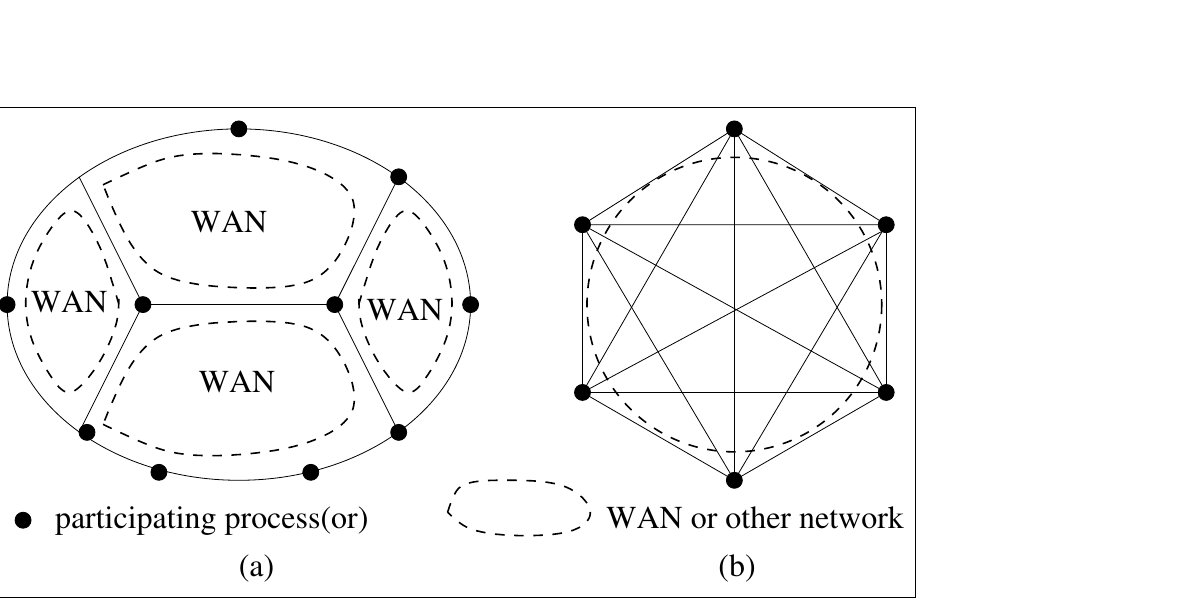
\includegraphics[width=.78\linewidth,height=.64\paperheight,keepaspectratio]{assets/week05-source-2025/topology-abstractions.png}
\end{center}
\smallnote{同一组参与进程可以被抽象成邻域视图，也可以被抽象成逻辑全连接；算法复杂度取决于采用的视图。}
\end{frame}

\begin{frame}{应用执行与控制算法执行}
\begin{columns}[T,onlytextwidth]
\column{.48\textwidth}
\blocktitle{应用执行}
\begin{itemize}
  \item 产生业务消息与业务状态；
  \item 目标是完成用户任务；
  \item 事件由应用语义解释。
\end{itemize}
\column{.48\textwidth}
\blocktitle{控制算法（协议）}
\begin{itemize}
  \item 监控、辅助和全局推理；
  \item 建树、MIS、CDS、共识、快照、检查点；
  \item 透明地叠加在应用执行之上。
\end{itemize}
\end{columns}
\vfill
\callout{设计要求}{控制算法的 send、receive、internal 事件尽量不改变应用的可观察语义。}
\end{frame}

\begin{frame}{集中式与分布式算法}
\begin{tabularx}{\linewidth}{>{\bfseries}p{2.5cm}XX}
\toprule
维度 & 集中式 & 分布式 \\
\midrule
角色 & 客户端--服务器，不对称 & 多节点角色更平衡 \\
瓶颈 & 处理、带宽和单点故障集中 & 设计复杂，需协调局部视图 \\
示例 & 单控制器全局计算 & 快照、树、MST、共识 \\
\bottomrule
\end{tabularx}
\vfill
\callout{经验}{“更分布式”不等于“更简单”；算法正确性往往来自额外的控制消息和不变量。}
\end{frame}

\begin{frame}{对称性：symmetric 与 asymmetric}
\begin{itemize}
  \item 对称算法：节点运行相同代码，初始状态也可能相同；
  \item 非对称算法：预先指定 root、leader、方向或角色；
  \item 很多全局算法需要一个 initiator 或 finisher；
  \item 若系统完全匿名且环对称，确定性选主不可能。
\end{itemize}
\vfill
\begin{center}\Large\color{ADSOrange}\bfseries 破除对称性：ID、随机数、方向、外部发起者。\end{center}
\end{frame}

\begin{frame}{Anonymous、uniform、adaptive}
\begin{tabularx}{\linewidth}{>{\bfseries}p{2.4cm}X}
\toprule
概念 & 约束与价值 \\
\midrule
Anonymous & 运行时决策不使用进程 ID；结构优雅，但匿名选主不可能。 \\
Uniform & 代码不把 $n$（进程总数）作为参数；节点加入/离开更容易。 \\
Adaptive & 令 $k\le n$ 为当前参与问题的节点数，复杂度用 $k$ 而非 $n$ 表示。 \\
\bottomrule
\end{tabularx}
\vfill
\callout{AI 基础设施}{弹性训练和在线服务更偏好 uniform/adaptive：扩缩容只需要邻居更新，而不是重写全局参数。}
\end{frame}

\begin{frame}{确定性与非确定性执行}
\begin{itemize}
  \item 确定性 receive 指定消息来源；
  \item 非确定性 receive 可以接收任意来源的下一条消息；
  \item 异步系统中，确定性程序重放通常保留相同事件偏序；
  \item 非确定性接收会因网络拥塞、CPU 调度和延迟变化产生不同偏序；
  \item 因此调试、稳定谓词检测和可复现实验需要记录调度信息。
\end{itemize}
\end{frame}

\begin{frame}{执行抑制（freezing）的两种分类}
\begin{columns}[T,onlytextwidth]
\column{.48\textwidth}
\blocktitle{按延迟事件的来源}
\begin{itemize}
  \item non-inhibitory：没有事件被协议禁用；
  \item locally inhibitory：延迟只由本地条件造成；
  \item globally inhibitory：某个延迟依赖远端 receive。
\end{itemize}
\column{.48\textwidth}
\blocktitle{按事件类型}
\begin{itemize}
  \item send-inhibitory；
  \item receive-inhibitory；
  \item internal-event-inhibitory。
\end{itemize}
\end{columns}
\vfill
\callout{分析问题}{协议等待控制消息时，冻结了应用哪一类事件？冻结成本是否影响吞吐和尾延迟？}
\end{frame}

\begin{frame}{同步与异步系统}
\begin{tabularx}{\linewidth}{>{\bfseries}p{2.2cm}XX}
\toprule
条件 & 同步系统 & 异步系统 \\
\midrule
消息延迟 & 有已知上界 & 无已知有限上界 \\
时钟漂移 & 相对真实时间有已知上界 & 不保证 \\
进程一步 & 有已知上界 & 不保证 \\
算法影响 & 可用轮次和超时终止 & 需显式 ACK、因果和稳定判定 \\
\bottomrule
\end{tabularx}
\vfill
\callout{在线/离线}{在线算法随数据生成执行，便于调度和故障诊断；离线算法先收集完整 trace，再统一处理。}
\end{frame}

\begin{frame}{Wait-free 与通信信道}
\begin{itemize}
  \item wait-free 同步操作能容忍最多 $n-1$ 个进程失败；
  \item 任一正确进程的操作都必须在有限步内完成，与其他进程是否停顿无关；
  \item 它很健壮，但实现通常昂贵；互斥可以做到，生产者--消费者未必总能做到；
  \item 点到点信道可为 FIFO 或 non-FIFO；应用层通常依赖网络栈提供 FIFO。
\end{itemize}
\end{frame}

\begin{frame}{进程故障模型：从 benign 到 Byzantine}
\begin{enumerate}
  \item fail-stop：进程停止，其他进程能获知；
  \item crash：进程停止，但不一定能获知；
  \item receive omission：只收到部分消息或崩溃；
  \item send omission：只发送部分消息或崩溃；
  \item general omission：send + receive omission；
  \item Byzantine：可任意行为、伪造或篡改消息；认证可验证“谁声称收到了什么”。
\end{enumerate}
\vfill
\callout{算法依赖}{故障模型越强，越不能把“没有消息”解释成“对方没有发送”。}
\end{frame}

\begin{frame}{链路故障与 timing failure}
\begin{itemize}
  \item link crash：链路停止传递消息；
  \item link omission：只丢失部分消息；
  \item link Byzantine：伪造、篡改或任意改变消息；
  \item timing failure：消息过快/过慢、时钟漂移超界或进程执行超时；
  \item 在同步系统中，timing failure 比 general omission 更严重。
\end{itemize}
\vfill
\begin{center}
\begin{tikzpicture}[node distance=8mm]
\nodebox{ADSBlue}{benign}{良性遗漏};
\nodebox[right=of benign]{ADSOrange}{timing}{时序故障};
\nodebox[right=of timing]{ADSGreen}{byz}{Byzantine};
\draw[ADSBlue,\arrow] (benign)--(timing);
\draw[ADSOrange,\arrow] (timing)--(byz);
\end{tikzpicture}
\end{center}
\end{frame}

\begin{frame}{复杂度：不要只报一个数字}
\begin{itemize}
  \item 每个指标都可用下界 $\Omega(\cdot)$、上界 $O(\cdot)$ 或精确界 $\Theta(\cdot)$ 表示；
  \item 节点空间与系统总空间不同，最坏情况未必同时发生在所有节点；
  \item 节点时间与系统时间不同，后者还取决于并发度；
  \item 消息复杂度既要数消息个数，也要考虑消息大小和并发发送/接收。
\end{itemize}
\end{frame}

\begin{frame}{复杂度度量表}
\begin{tabularx}{\linewidth}{>{\bfseries}p{3.1cm}X}
\toprule
指标 & 需要回答的问题 \\
\midrule
局部/系统空间 & 每个节点与全系统保存多少状态、缓存多少控制消息？ \\
局部/系统时间 & 单节点多久完成？所有节点何时都完成？ \\
消息数/大小 & 消息总数是多少？每条携带多少 ID、向量或整行数据？ \\
消息时间 & 发送、传输、排队和并发接收如何叠加？ \\
事件/同步操作 & send、receive、multicast、共享内存同步各发生多少次？ \\
\bottomrule
\end{tabularx}
\end{frame}

\begin{frame}{本讲算法地图}\small
\begin{columns}[T,onlytextwidth]
\column{.32\textwidth}
\begin{itemize}
  \item 同步/异步 1-init ST；
  \item 并发发起 ST；
  \item 异步 DFS ST；
  \item broadcast/convergecast。
\end{itemize}
\column{.32\textwidth}
\begin{itemize}
  \item Bellman--Ford；
  \item Floyd--Warshall；
  \item constrained flooding；
  \item GHS MST。
\end{itemize}
\column{.32\textwidth}
\begin{itemize}
  \item synchronizer；
  \item MIS / CDS；
  \item compact routing；
  \item leader election / replication。
\end{itemize}
\end{columns}
\vfill
\callout{共同范式}{局部状态 + 控制消息 + 终止条件 + 可证明不变量。}
\end{frame}

\sectionframe{二、生成树与树上聚合}{生成树是分布式算法的“控制骨架”：它把任意图上的全局传播变成树上的上下行。}

\begin{frame}{同步 1-init spanning tree：问题与假设}
\begin{itemize}
  \item 输入：连通无向图 $G=(N,L)$，预先指定 root；
  \item 每个进程只知道邻居集合，不知道全局图；
  \item 同步轮次使“距离 root 为 $r$ 的节点”在第 $r$ 轮看到 QUERY；
  \item 目标：每个节点选择一个 parent，所有 parent 边形成 spanning tree。
\end{itemize}
\vfill
\callout{直觉}{flooding 的第一条 QUERY 近似对应 BFS 的最短层级。}
\end{frame}

\begin{frame}{同步 flooding：局部变量与消息}
\begin{block}{状态}
$visited\in\{0,1\}$，$depth$，$parent$，以及邻居集合 $Neighbors$。
\end{block}
\begin{block}{消息}
唯一控制消息为 $QUERY$；root 在第 0 轮发送给所有邻居。
\end{block}
\begin{itemize}
  \item 未访问节点在收到本轮 QUERY 后任选一个发送者作为 parent；
  \item 向本轮未作为发送者的邻居继续转发；
  \item 每轮末删除本轮 QUERY，避免重复使用。
\end{itemize}
\end{frame}

\begin{frame}{同步 1-init ST：伪代码}
\scriptsize
\begin{block}{Synchronous flooding}
\begin{enumerate}
  \item 若 $i=root$：$visited\leftarrow1, depth\leftarrow0$，向 $Neighbors$ 发送 QUERY；
  \item 对 $round=1,\ldots,diameter$：
  \item \quad 若 $visited=0$ 且收到 QUERY，任选发送者 $j$，设 $parent\leftarrow j$、$depth\leftarrow round$；
  \item \quad 向 $Neighbors\setminus\{\text{本轮 QUERY 发送者}\}$ 发送 QUERY；
  \item \quad 删除本轮到达的 QUERY。
\end{enumerate}
\end{block}
\normalsize
\callout{终止}{同步系统按已知直径运行 $d$ 轮；不需要单独 ACK。}
\end{frame}

\begin{frame}{同步 ST 的例子}
\begin{center}
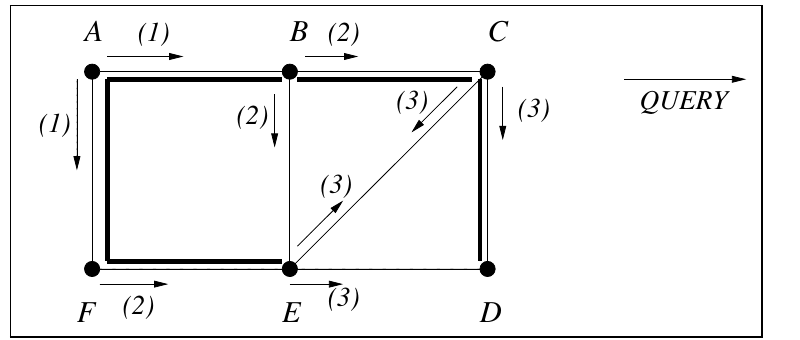
\includegraphics[width=.72\linewidth,height=.62\paperheight,keepaspectratio]{assets/week05-source-2025/sync-tree-example-full.png}
\end{center}
\smallnote{A 为指定 root，括号是 QUERY 到达的轮次；粗边为树边。孩子节点可通过“谁收到我的 QUERY 并返回 ACK”或记录邻居 parent 推断。}
\end{frame}

\begin{frame}{同步 ST：复杂度与 BFS 关系}
\begin{tabularx}{\linewidth}{>{\bfseries}p{3.2cm}X}
\toprule
终止 & $diameter$ 轮后完成 \\
局部空间 & $O(degree)$，保存邻居和 parent/visited \\
系统空间 & $O(\sum_i degree_i)$ \\
局部时间 & $O(degree+diameter)$ \\
消息复杂度 & 每条边 1--2 条消息，区间 $[|L|,2|L|]$ \\
\bottomrule
\end{tabularx}
\vfill
\callout{关系}{同步 flooding 生成的树与 BFS 树类似；同步性带来层级，但不自动解决孩子确认。}
\end{frame}

\begin{frame}{异步 1-init ST：为什么需要 ACCEPT/REJECT}
\begin{itemize}
  \item root 向所有邻居发送 QUERY；第一个 QUERY 到达的邻居成为 parent；
  \item 被接受的 QUERY 对应树边，返回 ACCEPT；
  \item 其他 QUERY 对应 cross/back edge，返回 REJECT；
  \item 节点只有收到所有非 parent 邻居的 ACCEPT/REJECT 才能本地终止；
  \item 如果已知邻居数且传输层能提供确认，REJECT 可以被隐式化，但终止判断更复杂。
\end{itemize}
\end{frame}

\begin{frame}{异步 1-init ST：状态与事件}
\begin{block}{局部变量}
$parent$，孩子集合 $Children$，非树邻居集合 $Unrelated$，$Neighbors$。
\end{block}
\begin{block}{消息}
$QUERY$、$ACCEPT$、$REJECT$。
\end{block}
\begin{itemize}
  \item parent 初始为未知；root 将自己的 parent 设为自己；
  \item QUERY 到达且 parent 未知时接受，否则拒绝；
  \item ACCEPT 加入 children，REJECT 加入 unrelated。
\end{itemize}
\end{frame}

\begin{frame}{异步 1-init ST：伪代码语义}
\scriptsize
\begin{enumerate}
  \item root：向所有邻居发 QUERY，$parent\leftarrow root$；
  \item 收到 QUERY(j)：若 $parent=?$，设 $parent\leftarrow j$，回 ACCEPT，并向除 $j$ 外的邻居发 QUERY；否则回 REJECT；
  \item 收到 ACCEPT(j)：$Children\leftarrow Children\cup\{j\}$；
  \item 收到 REJECT(j)：$Unrelated\leftarrow Unrelated\cup\{j\}$；
  \item 当 $Children\cup Unrelated=Neighbors\setminus\{parent\}$ 时终止。
\end{enumerate}
\normalsize
\vfill
\callout{不变量}{每条无向边最终要么被两端视为树边，要么被两端视为非树边。}
\end{frame}

\begin{frame}{异步 ST 的例子与消息类型}
\begin{columns}[T,onlytextwidth]
\column{.52\textwidth}
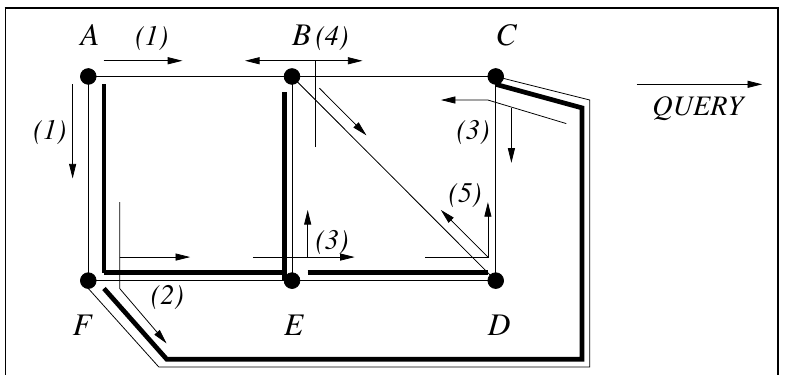
\includegraphics[width=\linewidth]{assets/week05-source-2025/async-tree-example-full.png}
\column{.44\textwidth}
\begin{itemize}
  \item 粗边：QUERY + ACCEPT；
  \item cross/back edge：QUERY + REJECT；
  \item QUERY 到达顺序决定 parent，不保证最短路径；
  \item 最坏树高可达 $n-1$。
\end{itemize}
\end{columns}
\end{frame}

\begin{frame}{异步 ST：复杂度}
\begin{tabularx}{\linewidth}{>{\bfseries}p{3.2cm}X}
\toprule
局部空间 & $O(degree)$ \\
系统空间 & $O(\sum_i degree_i)$ \\
局部时间 & $O(degree)$ 次本地响应 \\
消息复杂度 & 每条边 2--4 条消息，区间 $[2|L|,4|L|]$ \\
消息时间 & 最长路径 $d+1$ 个消息 hop \\
树高 & 无 BFS 保证，最坏 $n-1$ \\
\bottomrule
\end{tabularx}
\vfill
\callout{课堂追问}{能否不发 REJECT？代价是需要邻居枚举、超时或传输层 ACK；在纯异步模型中，沉默本身不是证据。}
\end{frame}

\begin{frame}{并发发起：多个 root 如何竞争}
\begin{center}
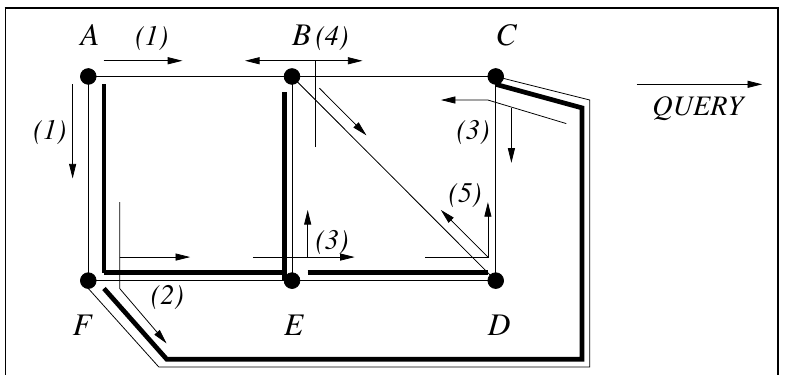
\includegraphics[width=.68\linewidth,height=.47\paperheight,keepaspectratio]{assets/week05-source-2025/async-tree-example-full.png}
\end{center}
\smallnote{并发发起的核心选择：合并多个局部 ST（可能产生环），或只让一个实例继续；一种规则是让更高 ID 的 root 压制更低 ID。}
\end{frame}

\begin{frame}{并发 initiator：newroot 规则}
\begin{itemize}
  \item 节点维护 $myroot$；初始 root 自发起并把自己作为 $myroot$；
  \item 收到 $QUERY(newroot)$：若 $newroot>myroot$，丢弃旧执行，更新 parent/myroot 并转发；
  \item 若 $newroot=myroot$，parent 已确定，返回 REJECT；
  \item 若 $newroot<myroot$，忽略 QUERY，发送更高 root 的消息会让对方更新；
  \item 只有最终获胜 root 检测全局终止，再沿 ST 通知其他节点。
\end{itemize}
\end{frame}

\begin{frame}{并发 initiator：复杂度与正确性}
\begin{itemize}
  \item 选最大的 root ID 后，所有节点最终收敛到同一个 $myroot$；
  \item 旧实例的部分边不会被当作最终树边；
  \item 时间复杂度 $O(d)$，但重复实例可能使消息复杂度达到 $O(n|L|)$；
  \item 终止通知是额外消息，不能把“局部稳定”误当成“全局完成”。
\end{itemize}
\vfill
\callout{AI 映射}{Kubernetes 控制器或 Ray driver 选 root 时，generation/epoch 可以充当 $newroot$ 的优先级。}
\end{frame}

\begin{frame}{异步 DFS spanning tree}
\begin{itemize}
  \item 并发 root 处理与非 DFS 版本相同：更高 root 压制低 root；
  \item 每个节点维护 $Unknown$ 邻居集合，一次只向一个未知邻居发送 QUERY；
  \item 收到 ACCEPT 才沿当前分支继续，REJECT 后尝试下一个未知邻居；
  \item root 只有在所有邻居都被探查后终止，并沿树发送完成通知；
  \item 时间 $O(d)$，消息复杂度 $O(n|L|)$。
\end{itemize}
\end{frame}

\begin{frame}{异步 DFS：完整中文伪代码（发起与 QUERY）}
\scriptsize
本地状态：$parent$、$myroot$、$Children$、$Neighbours$、$Unknown$；消息为 \texttt{QUERY/ACCEPT/REJECT}。
\begin{enumerate}
  \item 节点 $i$ 发起：若尚无 parent，向自己发送 \texttt{QUERY(i)}。
  \item 从 $j$ 收到 \texttt{QUERY(newroot)}：
    \begin{enumerate}
      \item 若 $newroot>myroot$：令 $parent\leftarrow j$、$myroot\leftarrow newroot$、$Unknown\leftarrow Neighbours\setminus\{j\}$；
      \item 若 $Unknown\neq\emptyset$，取出一个 $x$，仅向 $x$ 发送 \texttt{QUERY(myroot)}；否则向 $j$ 返回 \texttt{ACCEPT(myroot)}；
      \item 若 $newroot=myroot$，向 $j$ 返回 \texttt{REJECT(myroot)}；
      \item 若 $newroot<myroot$，忽略该旧执行消息。
    \end{enumerate}
\end{enumerate}
\smallnote{一次只探查一个 $Unknown$ 邻居，是 DFS 与并行 flooding 的根本差异。}
\end{frame}

\begin{frame}{异步 DFS：完整中文伪代码（ACCEPT/REJECT）}
\scriptsize
从 $j$ 收到 \texttt{ACCEPT(newroot)} 或 \texttt{REJECT(newroot)}：
\begin{enumerate}
  \item 只有 $newroot=myroot$ 时才处理；较旧 root 的回复全部丢弃。
  \item 若是 \texttt{ACCEPT}，令 $Children\leftarrow Children\cup\{j\}$；\texttt{REJECT} 只表示该边不是树边。
  \item 若 $Unknown\neq\emptyset$，取出下一个 $x$，发送 \texttt{QUERY(myroot)}，继续当前深度优先分支。
  \item 若 $Unknown=\emptyset$：
    \begin{enumerate}
      \item 若 $parent\neq i$，向 parent 返回 \texttt{ACCEPT(myroot)}，把整个已探索子树交还上一层；
      \item 若 $parent=i$，则 $i$ 是最终 root，算法终止。
    \end{enumerate}
\end{enumerate}
\callout{正确性直觉}{每个节点只接受最高 root 的一次父关系；每条候选边最终得到 ACCEPT 或 REJECT，因此树连通且不会形成环。}
\end{frame}

\begin{frame}{Broadcast 与 convergecast}
\begin{center}
\begin{tikzpicture}[scale=.82,transform shape,node distance=6mm and 10mm,>=Latex]
  \nodebox{ADSBlue}{br}{根};
  \nodebox[below left=of br]{ADSGray}{b1}{节点};
  \nodebox[below right=of br]{ADSGray}{b2}{节点};
  \nodebox[below=of b1]{ADSGray}{b3}{叶子};
  \nodebox[below=of b2]{ADSGray}{b4}{叶子};
  \draw[\arrow,ADSBlue] (br)--(b1);
  \draw[\arrow,ADSBlue] (br)--(b2);
  \draw[\arrow,ADSBlue] (b1)--(b3);
  \draw[\arrow,ADSBlue] (b2)--(b4);
  \node[below=6mm of $(b3)!0.5!(b4)$,ADSBlue]{Broadcast：自上而下复制};
  \begin{scope}[xshift=6.5cm]
    \nodebox{ADSOrange}{cr}{根};
    \nodebox[below left=of cr]{ADSGray}{c1}{聚合};
    \nodebox[below right=of cr]{ADSGray}{c2}{聚合};
    \nodebox[below=of c1]{ADSGray}{c3}{叶子};
    \nodebox[below=of c2]{ADSGray}{c4}{叶子};
    \draw[\arrow,ADSOrange] (c3)--(c1);
    \draw[\arrow,ADSOrange] (c4)--(c2);
    \draw[\arrow,ADSOrange] (c1)--(cr);
    \draw[\arrow,ADSOrange] (c2)--(cr);
    \node[below=6mm of $(c3)!0.5!(c4)$,ADSOrange]{Convergecast：自下而上汇聚};
  \end{scope}
\end{tikzpicture}
\end{center}
\smallnote{树边提供无环骨架；broadcast 自上而下，convergecast 自下而上。环或 mesh 需要先建树或额外去重。}
\end{frame}

\begin{frame}{树上的 BC/CC 规则与成本}
\begin{columns}[T,onlytextwidth]
\column{.47\textwidth}
\blocktitle{Broadcast}
\begin{itemize}
  \item root 向所有孩子发送信息；
  \item 非 root 收到 parent 信息后复制并转发；
  \item 时间 $O(h)$，消息数 $n-1$。
\end{itemize}
\column{.47\textwidth}
\blocktitle{Convergecast}
\begin{itemize}
  \item 叶子先上报；
  \item 非叶等待所有孩子，聚合后上报；
  \item root 计算 min、max、leader 或全局状态；
  \item 时间 $O(h)$，消息数 $n-1$。
\end{itemize}
\end{columns}
\vfill
\callout{AI 基础设施}{训练集群的梯度 all-reduce、参数广播和日志汇总，都可以拆成树上的 BC/CC。}
\end{frame}

\latercontent
\begin{frame}{算法边界卡：结论只在对应模型内成立}
\small
\begin{tabularx}{\linewidth}{>{\bfseries}p{3.0cm}XX}
\toprule
Bellman--Ford & 本例按同步轮次传播，且假设不存在负权环；异步距离向量还要处理旧信息与 count-to-infinity。 & “距离暂时不再变化”不等于在任意动态网络中已经收敛。 \\
同步化 GHS & 采用 Borůvka 风格的教学化轮次；标准 GHS 是带 level/phase 的异步协议。 & 课件中的轮数和消息量不能直接称为标准 GHS 的复杂度。 \\
分布式 Floyd--Warshall & 所有节点必须按同一 pivot 阶段推进并拿到对应 pivot 行。 & 若节点混用不同阶段的数据，三角不等式仍能计算，但不再保持算法不变量。 \\
Synchronizer & 通过 ACK、树和安全点模拟同步轮次，通常先假设无故障。 & 故障和网络分区需要额外的重配置或故障检测机制。 \\
\bottomrule
\end{tabularx}
\vfill
\callout{解题习惯}{先写“同步/异步、可靠/丢失、是否知道 $n$、是否有动态拓扑”，再写算法步骤与复杂度。}
\end{frame}
\end{document}
